\documentclass[aspectratio=169]{beamer}
\usepackage{graphicx}
\usepackage{booktabs}
\graphicspath{{../report/figures/}}
\definecolor{ctxindigo}{HTML}{4F46E5}
\setbeamercolor{structure}{fg=ctxindigo}
\setbeamercolor{frametitle}{fg=ctxindigo}
\setbeamercolor{title}{fg=white,bg=ctxindigo}
\setbeamercolor{author}{fg=white}
\setbeamercolor{date}{fg=white}
\setbeamertemplate{navigation symbols}{}
\newcommand{\src}[1]{{\footnotesize\textcolor{gray}{#1}}}

\title{CtxVigil --- DA2 Review\\Results and Evaluation Metrics}
\author{Rishabh Tripathi (24BRS1136) \quad Saumya (24BRS1065)\\ \footnotesize Course BCSE306L --- Artificial Intelligence}
\date{}

\begin{document}

\begin{frame}
\titlepage
\end{frame}

\begin{frame}{Four evaluation surfaces, all reproducible}
\begin{enumerate}
  \item \textbf{DeBERTa-v3 classifier} --- metrics on the 3{,}000-sample held-out test set (Colab Notebook 1, cell 9).
  \item \textbf{Fusion \& uncertainty network} --- metrics on the 1{,}000 held-out episodes (Colab Notebook 2, cell 9; exported summary artifact).
  \item \textbf{Rule-based layer} --- 7 contract fixtures with declared expected verdicts (\texttt{packages/ctxvigil-core} test suite).
  \item \textbf{Live agent episodes} --- 6 end-to-end runs with verdict assertions and latency measurement (\texttt{npm run agent:demo}).
\end{enumerate}
Every number in this deck was produced by one of those four runs and can be re-derived from the repository.
\end{frame}

\begin{frame}{DeBERTa-v3 classifier --- held-out test set (3{,}000 samples)}
\begin{center}
\begin{tabular}{@{}lr@{}}
\toprule
\textbf{Metric} & \textbf{Value} \\
\midrule
Accuracy & 100.00\% \\
Precision & 100.00\% \\
Recall & 100.00\% \\
F1-score & 100.00\% \\
ROC-AUC & 1.000 \\
\bottomrule
\end{tabular}
\end{center}
\begin{itemize}
  \item The hard negatives (benign sentences containing ``ignore'' / ``override'' / ``system'') are classified correctly --- the model reads intent, not keywords.
  \item Exported artifact: \texttt{notebooks/exports/deberta\_test\_inferences.csv} (per-sample labels and probabilities) + \texttt{ctxvigil\_viva\_summary.json}.
\end{itemize}
\src{Colab Notebook 1, cell 9 (prints this exact table) · summary JSON in notebooks/exports/.}
\end{frame}

\begin{frame}{Confusion matrix and ROC (exported test sample)}
\begin{columns}
\begin{column}{0.48\textwidth}
\begin{center}
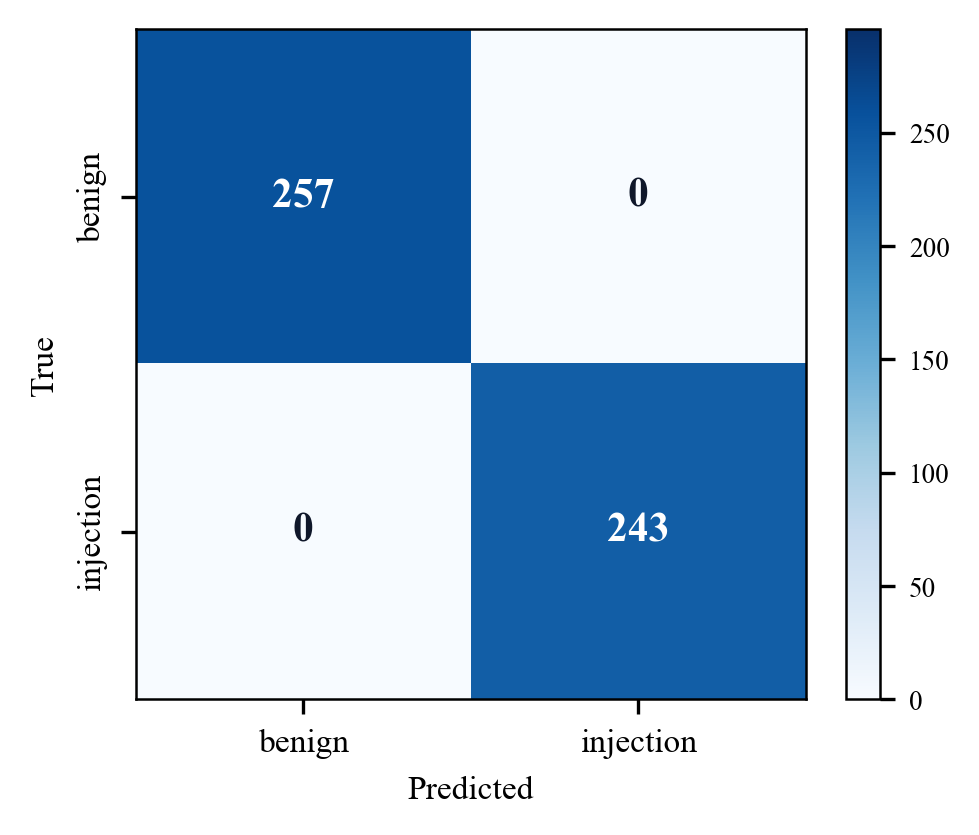
\includegraphics[width=\textwidth]{fig3_confusion_matrix.png}
\end{center}
\end{column}
\begin{column}{0.48\textwidth}
\begin{center}
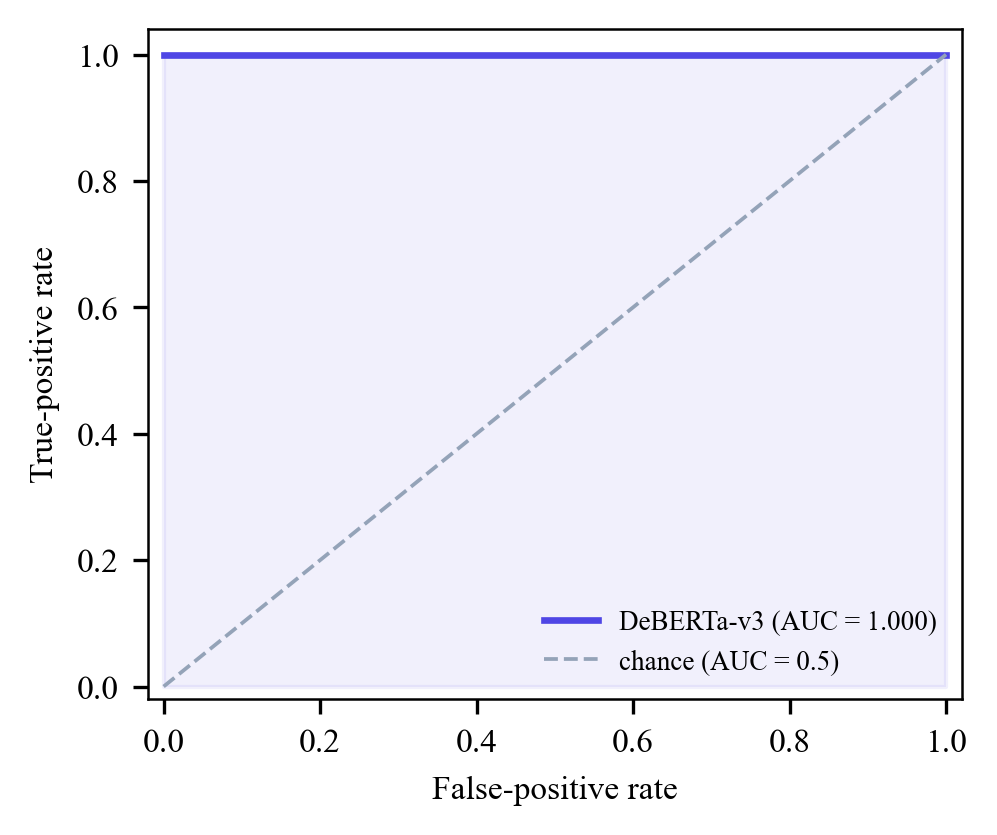
\includegraphics[width=\textwidth]{fig4_roc.png}
\end{center}
\end{column}
\end{columns}
\src{Computed from notebooks/exports/deberta\_test\_inferences.csv (500-row exported sample: 243 injection, 257 benign): 0 false positives, 0 false negatives.}
\end{frame}

\begin{frame}{Score separation (why the ROC is perfect)}
\begin{columns}
\begin{column}{0.5\textwidth}
\begin{center}
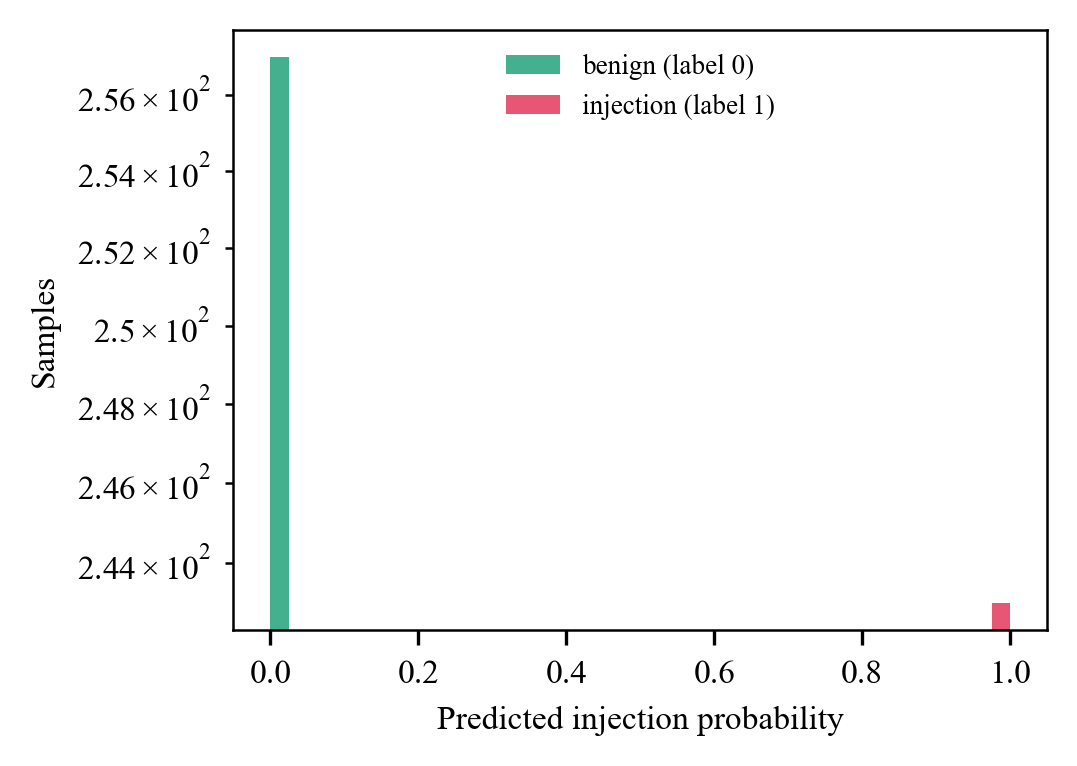
\includegraphics[width=\textwidth]{fig5_prob_separation.png}
\end{center}
\end{column}
\begin{column}{0.5\textwidth}
\begin{itemize}
  \item Predicted probabilities are saturated: benign mass at 0.0, injection mass at 1.0, no mass at the boundary.
  \item Perfect separation on a \emph{template-derived} benchmark is expected and is reported honestly as such (see limitations slide) --- the deployable system does not rely on it for enforcement.
\end{itemize}
\end{column}
\end{columns}
\src{Same exported CSV; histogram of \texttt{predicted\_prob} by true label.}
\end{frame}

\begin{frame}{Fusion \& uncertainty network --- 1{,}000 held-out episodes}
\begin{center}
\begin{tabular}{@{}lr@{}}
\toprule
\textbf{Metric} & \textbf{Value} \\
\midrule
Risk accuracy & 100\% \\
Precision / Recall & 100\% / 100\% \\
F1-score & 100\% \\
ROC-AUC & 1.000 \\
Model size & 1.6 MB (MLP weights) \\
\bottomrule
\end{tabular}
\end{center}
\begin{itemize}
  \item Trained with the dual objective $\mathcal{L} = \mathcal{L}_{\mathrm{CE}}(\text{risk}) + 0.5\,\mathcal{L}_{\mathrm{MSE}}(\text{uncertainty})$ --- 15 epochs, AdamW, batch 64.
  \item Live simulation (Notebook 2, cell 11): a benign order query $\rightarrow$ \textbf{ALLOW}; the InjecAgent hijack ($p_{\mathrm{DeBERTa}} = 0.98$) $\rightarrow$ \textbf{BLOCK}; boundary cases route to \textbf{QUARANTINE} (human confirmation).
\end{itemize}
\src{Exported summary: notebooks/exports/ctxvigil\_viva\_summary.json · training in Colab Notebook 2, cells 8--9.}
\end{frame}

\begin{frame}{Rule-based layer --- 7 contract fixtures}
\begin{center}
\footnotesize
\begin{tabular}{@{}lrrl@{}}
\toprule
\textbf{Fixture} & \textbf{Score} & \textbf{Scan} & \textbf{Gate} \\
\midrule
safe-refund-page & 0 & allow & allow \\
visible-injection & 65 & confirm & confirm \\
hidden-dom-injection & 95 & block & block \\
aria-injection & 100 & block & block \\
benign-aria-label & 0 & allow & allow \\
unrelated-account-action & 0 & allow & \textbf{block} \\
task-aligned-summary-action & 0 & allow & allow \\
\bottomrule
\end{tabular}
\end{center}
\textbf{All 7 assertions pass.} Note the two headline behaviours: the hidden ARIA injection scores 100 although nothing is visible on screen, and the unrelated account change is caught by the \emph{gate} on a page that scans clean.
\src{packages/ctxvigil-core/tests (contract tests) · tests/results/observed-contract-results.json · chart: fig6 in the report figures.}
\end{frame}

\begin{frame}{Live agent episodes --- verdicts and latency (systems metrics)}
\begin{center}
\footnotesize
\begin{tabular}{@{}lrr@{}}
\toprule
\textbf{Episode} & \textbf{Latency (ms)} & \textbf{Gate} \\
\midrule
aria-injection & 21 & block \\
injecagent-indirect-hijack & 3 & block \\
visible-injection & 2 & confirm \\
task-deviation-settings & 3 & block \\
benign-aria-negative & 2 & allow \\
safe-refund-page & 2 & allow \\
\midrule
\textbf{All six episodes} & \textbf{33} & \textbf{6/6 assertions pass} \\
\bottomrule
\end{tabular}
\end{center}
Per-episode end-to-end latency 2--21\,ms on a commodity laptop \textbf{CPU}, fully offline --- the deterministic enforcement adds negligible overhead to the agent loop. (The LLM-driven chat demo adds Gemini round-trips on top of the same layer.)
\src{Recorded run: apps/demo-web/public/agent-runs/latest.json · reproduce with \texttt{npm run agent:demo}.}
\end{frame}

\begin{frame}{Honest limitations (say this to the faculty)}
\begin{itemize}
  \item The 100\% classifier and fusion scores are on \textbf{template-derived} datasets: they demonstrate separation on the attack families the benchmark was designed around, not robustness to arbitrary novel injections.
  \item Therefore the deployment keeps enforcement in the \textbf{deterministic, explainable layer} (contract-tested, 2--21\,ms) and treats the learned models as \textbf{advisory} signals --- the ML can never weaken the guarantees.
  \item Rule-layer limits: phrase tables must be maintained; semantically novel phrasing is caught by the gate's alignment/posture axes rather than the scan.
  \item Next step: evaluate the learned components on external benchmarks (full InjecAgent, AgentDojo) and calibrate the fusion output as a score calibrator behind the same policy interface.
\end{itemize}
\end{frame}

\begin{frame}{Verify everything yourself}
\begin{itemize}
  \item \texttt{npm run agent:demo} --- replays all six fixture pages through the real SDK, prints every verdict, asserts 6/6.
  \item \texttt{npm test} (in \texttt{packages/ctxvigil-core}) --- 145 tests incl.\ the 7 contract fixtures.
  \item \texttt{notebooks/exports/} --- per-sample test inferences (CSV) and the metrics summary (JSON).
  \item Colab Notebooks 1 and 2 --- every dataset figure and metric in this deck is printed by a notebook cell; re-running regenerates all of it.
  \item IEEE report with the same results: \texttt{submission/report/ctxvigil\_da2\_report.pdf}.
\end{itemize}
\end{frame}

\end{document}
